\section{Hoạt động thực hành trải nghiệm}
\subsection{Tóm tắt lý thuyết}
\subsubsection{Ước tính số cá thể trong quần thể}
Trong nghiên cứu về những quần thể động vật, một vấn đề quan trọng là ước tính số cá thể trong quần thể. Một phương pháp được sử dụng là đánh dấu và bắt lại.\\
Phương pháp: 
\begin{enumerate}
	\item Chọn $M$ cá thể từ quần thể, đánh dấu và thả chúng trở lại quần thể.
	\item Sau một thời gian, chọn ngẫu nhiên $n$ cá thể trong quần thể. Gọi $k$ là số cá thể được đánh dấu trong $n$ cá thể đó.\\
	Khi đó, xét phép thử: Chọn ngẫu nhiên một cá thể từ quần thể và xét biến cố $A$: \lq\lq  Cá thể có được đánh dấu\rq\rq. Gọi $N$ là số cá thể trong quần thể, khi đó xác suất của $A$ là $\mathrm{P}(A)=\dfrac{M}{N}$.\\
	Trong $n$ cá thể được chọn số cá thể được đánh dấu là $k$ xấp xỉ với $n\cdot \mathrm{P}(A)=n\cdot \dfrac{M}{N}$. Do đó $N$ được tính bởi công thức 
	\[N\approx M\cdot \dfrac{n}{k}.\]
\end{enumerate}
\subsubsection{Hoạt động trải nghiệm nội dung hình học}
Trong trải nghiệm nội dung hình học, ta thường sử dụng các định lý sau
\begin{enumerate}
\item Định lý sin ``Trong tam giác $ABC$ có $\dfrac{a}{\sin A}=\dfrac{b}{\sin B}=\dfrac{c}{\sin C}=2R$.''
\item Định lý Cô-sin ``Trong tam giác $ABC$ có các khẳng định sau
\begin{itemize}
\item $a^{2}=b^{2}+c^{2}-2 \cdot b \cdot c \cdot \cos A$.
\item $b^{2}=a^{2}+c^{2}-2 \cdot a \cdot c \cdot \cos B$.
\item $c^{2}=a^{2}+b^{2}-2 \cdot a \cdot b \cdot \cos C$.''
\end{itemize}
\end{enumerate}

\subsubsection{Tiết kiệm \& đầu tư}
		Gửi $A$ đồng vào ngân hàng với lãi suất kép $r\%$/năm, sau $n$ năm, số tiền nhận được tính theo công thức:
		$$T = A (1+r\%)^n$$
\subsubsection{Thuế thu nhập cá nhân}
		\begin{itemize}
		\item Thuế thu nhập cá nhân là khoản tiền (thuế) mà người có thu nhập phải trích nộp một phần vào ngân sách nhà nước sau khi đã tính các khoản được giảm trừ. Các khoản giảm trừ thông thường bao gồm:
		\begin{itemize}
		\item Giảm trừ bản thân;
		\item Giảm trừ người phụ thuộc.
		\end{itemize}
		\item Thuế suất thuế thu nhập cá nhân là tỉ lệ phần trăm dùng để tính số thuế phải nộp căn cứ vào phần thu nhập tính thuế của mỗi người.
		\item Thu nhập tính thuế $=$ Thu nhập chịu thuế $-$ Các khoản giảm trừ.
		\item Thuế thu nhập cá nhân $=$ Thu nhập tính thuế $\times$ Thuế suất.
		\end{itemize}
	
\subsection{Các ví dụ minh họa}
\begin{dang}{Ước tính số cá thể}
	Dựa vào công thức ước tính số cá thể để xác định số cá thể trong quần thể ở một số trường hợp nhất định
		\[N\approx M\cdot \dfrac{n}{k},\]
	trong đó $M$ là số cá thể đánh dấu, $n$ là số cá thể bắt lại, $k$ là số cá thể có đánh dấu trong $n$ cá thể bắt lại.
\end{dang}
\viduminhhoa
\begin{vd}
	Ước tính số lượng cá trong hồ. Biết rằng, lần thứ nhất người ta đánh bắt được $1500$ con và đánh dấu chúng, sau đó thả lại xuống hồ. Lần thứ hai người ta đánh bắt được $1800$ con và nhận thấy trong $1800$ con đó có $100$ con được đánh dấu.
	\loigiai{
	Ta có $M=1500$; $n=1800$; $k=100$.\\
	Khi đó ước lượng số cá trong hồ ta được kết quả là $N\approx 1500\cdot \dfrac{1800}{100}=27000$ (con).
}  
\end{vd}
\begin{vd}
	Ước tính số lượng lạc có trong túi. Biết rằng:
	\begin{enumerate}
	\item Lấy ra một cốc lạc trong túi, thấy có $ 85 $ hạt và đánh dấu chúng.
	\item Đổ số lạc đã được đánh dấu vào lại trong túi và xáo trộn đều.
	\item Lấy ra nửa cốc lạc, thấy có $ 43 $ hạt lạc và số hạt lạc có đánh dấu là $6$.
	\end{enumerate}
\loigiai{
Ta có $M=85$; $n=43$; $k=6$.\\
Khi đó ước lượng số hạt lạc có trong túi, ta được kết quả là $N\approx 85\cdot \dfrac{43}{6}\approx 609$ (hạt).
}
\end{vd}

\begin{vd}
	Trong tiết thực hành trải nghiệm của lớp 10A, tổ của Hà đã thực hiện các bước để ước lượng số lạc có trong túi. Tuy nhiên, lại lặp lại bước 3 thêm hai lần: lần hai lấy $ 1 $ cốc lạc, lần ba lấy $1{,}5$ cốc lạc và thu được kết quả như sau: 
	\begin{center}
		\begin{tabular}{|c|c|c|}
			\hline 
			Lần thứ & Số hạt $(n)$ & Số hạt có đánh dấu $(k)$\\
			\hline 
			$1$ & $51$ & $4$\\
			\hline 
			$2$ & $103$ & $11$\\
			\hline 
			$3$ & $155$ & $16$\\
			\hline 
		\end{tabular}
	\end{center}
Giả sử số hạt lạc trong túi đựng là $N=1000$ và số hạt được đánh dấu là $M=100$. Kí hiệu $\widehat{N}$ là số quy tròn đến hàng đơn vị của đại lượng $M\cdot \dfrac{n}{k}$.
\begin{enumEX}{1}
	\item Dựa vào dữ liệu, hãy hoàn thành bảng tính theo mẫu sau:
	\begin{center}
		\begin{tabular}{|c|c|c|c|c|c|c|c|}
			\hline 
			Lần & $N$ & $M$ & $n$ & $k$ & $\widehat{N}$ & Sai số tuyệt đối & Sai số tương đối\\
			\hline
			$1$ & $1000$ & $100$ & $51$ & $4$ & $ ? $ & ? & ?\\
			\hline
			$2$ & $1000$ & $100$ & $?$ & $?$ & ? & ? & ?\\
			\hline
			$3$ & $1000$ & $100$ & $?$ & $?$ & ? & ? & ?\\
			\hline
		\end{tabular}
	\end{center}
\item Em có nhận xét gì về sai số của việc tính xấp xỉ số hạt lạc trong túi khi $n$ càng lớn?
\end{enumEX}
\loigiai{
\begin{enumerate}
	\item 
	$ $ 
	\begin{center}
		\begin{tabular}{|c|c|c|c|c|c|c|c|}
			\hline 
			Lần & $N$ & $M$ & $n$ & $k$ & $\widehat{N}$ & Sai số tuyệt đối & Sai số tương đối\\
			\hline
			$1$ & $1000$ & $100$ & $51$ & $4$ & $ 1275 $ & $0$ & $0$\\
			\hline
			$2$ & $1000$ & $100$ & $103$ & $11$ & $ 936 $ & $ 0{,}36$ & $0{,}038\%$\\
			\hline
			$3$ & $1000$ & $100$ & $155$ & $16$ & $ 969 $ & $ 0{,}25 $ & $0{,}026\%$\\
			\hline
		\end{tabular}
	\end{center}
\item Khi $n$ càng lớn thì sai số trong việc tính xấp xỉ số hạt lạc trong túi sẽ càng nhỏ.
\end{enumerate}
}
\end{vd}

\begin{dang}{Kiểm tra tính đúng đắn của một kết quả hình học thông qua những ví dụ cụ thể}
	Sử dụng các thước đo độ dài, góc và máy tính bỏ túi, có thể kiểm tra:
	 \begin{itemize}
	 	\item Định lý sin đối với một tam giác nội tiếp trong một đường tròn.
	 	\item Định lý cô-sin đối với một tam giác.
	 	\item Đẳng thức $ah_{a}=2\sqrt{p(p-a)(p-b)(p-c)}$ đối với tam giác $ABC$ với $a$, $b$, $c$ là độ dài ba cạnh tam giác, $p$ là nửa chu vi.
	 \end{itemize}
\end{dang}
\viduminhhoa

\begin{vd}
 	\immini{Cho tam giác $ABC$ như hình vẽ, có $AC=1{,}9 cm$, $BC=3{,}9 cm$, $\widehat{BCA}=69^{\circ}$.
 		\begin{enumerate}
 			\item Tính độ dài cạnh $AB$ và kiểm tra tính chính xác bằng thước đo độ dài.
 			\item Tính số đo góc $\widehat{BAC}$  và kiểm tra tính chính xác bằng thước đo độ.
 			\item Tính chiều cao $h_{a}$ của tam giác $ABC$ và kiểm tra tính chính xác bằng thực đó.
 		\end{enumerate}
}{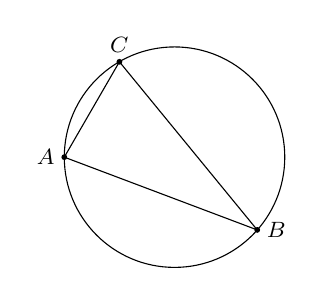
\begin{tikzpicture}[scale=0.7, line join=round, line cap=round,font=\footnotesize,>=stealth]	
	\path (0,0)coordinate[label=center:$ $](O) (-2,0)coordinate[label=left:$A$](A) (1.5,-1.32)coordinate[label=right:$B$](B) (-1,1.73)coordinate[label=above:$C$](C) ;
	

\draw[line width=0.4pt,black] (O) circle (2cm);
\draw[line width=0.4pt,black] (A)--(B)--(C)--(A);
		\fill[black] (A)circle(1.5pt);
		\fill[black] (B)circle(1.5pt);
		\fill[black] (C)circle(1.5pt);
\end{tikzpicture}
}
\loigiai{
\begin{enumerate}
	\item Áp dụng định lý cô-sin trong tam giác $ABC$ ta có
	\begin{eqnarray*}
		AB=\sqrt{AC^{2}+BC^{2}-2\cdot AC \cdot BC \cdot \cos C}=\sqrt{1{,}9^{2}+3{,}9^{2}-2\cdot 1{,}9 \cdot 3{,}9 \cdot \cos 69^{\circ}}\approx 3{,}7 cm.
	\end{eqnarray*}
Dùng thước đo độ dài, ta cũng đo được $AB \approx 3{,}7 cm$.
	\item Áp dụng định lý sin trong tam giác $ABC$ ta có \\
	\begin{center}
		$\dfrac{BC}{\sin A}=\dfrac{AB}{\sin C} \Rightarrow \sin A= \dfrac{BC \cdot \sin C}{AB}= \dfrac{3{,}9 \cdot \sin 69^{\circ}}{3{,}7} \approx 0{,}98$.
	\end{center}
Suy ra  $\widehat{BAC} \approx 79{,}8 ^{\circ}$.\\
Dùng thước đo độ, ta đũng đo được $\widehat{BAC} \approx 79{,}8 ^{\circ}$.
	\item Ta có 
	$S=\dfrac{1}{2}ah_{a}=\sqrt{p(p-a)(p-b)(p-c)}$, với 
	\begin{center}
	$p=\dfrac{a+b+c}{2}=\dfrac{BC+AC+AB}{2}=\dfrac{3{,}9+3{,}7+1{,}9}{2}=4{,}75$.
	\end{center}  
nên $ah_{a}=2\sqrt{p(p-a)(p-b)(p-c)}$.\\
	Suy ra 
	\begin{center}
		$3{,}9 \cdot h_{a}=2\sqrt{4{,}75(4{,}75-3{,}9)(4{,}75-3{,}7)(4{,}75-1{,}9)} \Rightarrow h_{a} \approx 1{,}8$.
	\end{center}
Sử dụng thước đo chiều dài, ta cũng đo được  $h_{a} \approx 1{,}8 cm$.
\end{enumerate}
}
  \end{vd}

\begin{dang}{Sử dụng kết quả hình học để tính toán trong đo đạc thực tế}
Sử dụng các định lý, hệ thức lượng trong tam giác khi tính toán số đo thực tế.
\end{dang}

\viduminhhoa

\begin{vd}
Đo chiều cao của một cái tháp mà không thể đến được chân tháp.
\loigiai{
\begin{itemize}
	\item \textit{Bước 1. Tìm hiểu yêu cầu bài toán}: Đo chiều cao của một cái tháp.
	\item \textit{Bước 2. Xây dựng mô hình toán học và giải bài toán}:
Lấy hình ảnh cụ thể để minh họa: mô hình cái tháp.\\
% TODO: \usepackage{graphicx} required
\begin{center}
	\includegraphics{images/hinh-thaptex-1}
\end{center}
	Giả sử $CD=h$ là chiều cao của tháp trong đó $C$ là chân tháp. \\
	Chọn hai điểm $A$, $B$ trên mặt đất sao cho ba điểm $A$, $B$ và $C$ thẳng hàng. \\
	Ta đo khoảng cách $AB$ và các góc $\widehat{CAD}$, $\widehat{CBD}$.
	\item \textit{Bước 3. Tiến hành đo đạc để lấy số liệu}:
Sử dụng thước đo chiều dài để đo khoảng cách hai điểm $A$ và $B$, ta được $AB=24m$.\\
Sử dụng giác kế để đo hai góc của tam giác $ABC$ là $\widehat{CAD} = \alpha=63^{\circ}$, $\widehat{CBD}=\beta=48^{\circ}$.
	\item \textit{Bước 4. Tính toán trên số liệu đo được}: Áp dụng định lý Sin vào tam giác $ABD$ ta có
	\begin{center}
	$	\dfrac{AD}{\sin \beta}=\dfrac{AB}{\sin D}$
	\end{center}
Ta có $\alpha =\widehat{D}+ \beta$ nên $\widehat{D}=\alpha- \beta=63^{\circ}-48^{\circ}=15^{\circ}$.\\
Do đó
\begin{center}
 $AD=\dfrac{AB \cdot \sin \beta }{\sin(\alpha -\beta)}=\dfrac{24 \cdot \sin 48^{\circ}}{\sin 15^{\circ}} \approx 68{,}91m$.
\end{center}
Trong  tam giác vuông $ACD$ ta có $h=CD=AD \sin \alpha \approx 61{,}4 m$.
\end{itemize}
}
	\end{vd}

	\begin{vd}
	Đo chiều rộng của một ao cá.
	\loigiai{
		\begin{itemize}
			\item \textit{Bước 1.Tình hiểu yêu cầu bài toán}:\\	Đo chiều rộng của một ao cá.
			\item \textit{Bước 2. Xây dựng mô hình toán học và giải bài toán}:\\ Lấy hình ảnh cụ thể để minh họa: hình ảnh ao cá.\\		
% TODO: \usepackage{graphicx} required
\begin{center}
	\includegraphics{images/hinh-boaotex-2}
\end{center}
		Gọi $d$ là chiều rộng (\textit{mặt nước}) ao cần đo. \\
			Xây dựng tam giác $ABC$ như hình. \\
		Chọn điểm $B$ là điểm bờ kẻ đá ở phía bên kia bờ ao đoạn ta khảo sát đo đạc để biết rộng của ao.\\
		Chọn điểm $A$ ở vị trí bờ ao đoạn ta khảo sát đo đạc để biết chiều rộng của ao, điểm $A$ bờ kẻ đá bên này ao.\\  
		Phía bờ ao có chọn điểm $A$ ta chọn tiếp $C$.
			\item \textit{Bước 3. Tiến hành đo đạc để lấy số liệu}:\\
			Sử dụng thước đo chiều dài để đo khoảng cách hai điểm $A$ và $C$, ta được $AC=55m$.\\
			Sử dụng giác kế để đo hai góc của tam giác $ABC$ là $\widehat{BAC} = 125{,}5^{\circ}$, $\widehat{BCA}= 48{,}5^{\circ}$.
			\item \textit{Bước 4. Tính toán trên số liệu đo được}:\\ Áp dụng định lý Sin vào tam giác $ABC$ ta có
			\begin{center}
				$	\dfrac{AC}{\sin B}=\dfrac{AB}{\sin C} \Rightarrow AB=\dfrac{AC \cdot \sin C }{\sin B}=\dfrac{55 \cdot \sin 48{,}5^{\circ}}{\sin (180^{\circ}-48{,}5^{\circ}-125{,}5^{\circ})} \approx 394{,}08 m$.
			\end{center}
		\end{itemize}
	}
\end{vd}

	\begin{vd}
	Bài toán khảo cổ học.\\
% TODO: \usepackage{graphicx} required
\begin{center}
	\includegraphics{images/hinh-diatex-4}
\end{center}
	Khi khai quật một ngôi mộ cổ, người ta tìm được một mảnh của 1 chiếu đĩa phẳng hình tròn bị vỡ. Dựa vào các tài liệu đã có, các nhà khảo cổ đã biết hình vẽ trên phần còn lại của chiếc đĩa. Họ muốn tìm một chiếc đĩa với phỏng theo chiếc đĩa này. Em hãy giúp họ tìm bán kính chiếc đĩa.
	\loigiai{
		\begin{itemize}
			\item \textit{Bước 1.Tình hiểu yêu cầu bài toán}: Tìm bán kính của chiếc đĩa.
			\item \textit{Bước 2. Xây dựng mô hình toán học và giải bài toán}:\\
			 Lấy hình ảnh cụ thể để minh họa.			
		Lấy 3 điểm $A$, $B$, $C$ trên cung tròn (\textit{mép đĩa}). Bài toán trở thành tìm $R$ khi biết $a$, $b$, $c$. \\
		Ta có $S=\sqrt{p(p-a)(p-b)(p-c)}$, $p=\dfrac{a+b+c}{2}$.\\
		$S=\dfrac{abc}{4R} \Rightarrow R=\dfrac{abc}{4S}$.
			\item \textit{Bước 3. Tiến hành đo đạc để lấy số liệu}:\\
			Ta có $AB=4{,}3 cm$; $BC=3{,}7 cm$; $AC=7{,}5 cm$.
			\item \textit{Bước 4. Tính toán trên số liệu đo được}: \\
			Xét tam giác $ABC$ ta có $p=\dfrac{AB+AC+BC}{2}=\dfrac{4{,}3+3{,}7+7{,}5}{2}=7{,}75cm$.\\
		Ta có\\
		$S=\sqrt{p(p-a)(p-b)(p-c)}=\sqrt{7{,}75(7{,}75-4{,}3)(7{,}75-3{,}7)(7{,}75-7{,}5)}=27{,}07$.\\
		$S=\dfrac{abc}{4R} \Rightarrow R=\dfrac{abc}{4S}=\dfrac{4{,}3 \cdot 3{,}7\cdot 7{,}5}{4\sqrt{27{,}07}}=5{,}7 cm$.

		\end{itemize}
Bài toán khảo cổ học mà còn có thể dùng trong công nghiệp thực phẩm (Chế tạo hộp đựng bánh qui, chế tạo bánh quy theo mẫu là 1 phần bánh qui), trong công nghiệp chế tạo máy (làm lại phần bị hỏng của bánh xê, bánh lái tàu,...),...
	}
\end{vd}

\begin{vd}
	Đo khoảng cách giữa hai điểm ở hai bờ đầm lầy để xây cầu. 
	\loigiai{
		\begin{itemize}
			\item \textit{Bước 1.Tình hiểu yêu cầu bài toán}:\\		Đo khoảng cách giữa hai điểm ở hai bờ đầm lầy.
			\item \textit{Bước 2. Xây dựng mô hình toán học và giải bài toán}:\\ Lấy hình ảnh cụ thể để minh họa
% TODO: \usepackage{graphicx} required
\begin{center}
	\includegraphics{images/hinh-damlaytex-3}
\end{center}
			Gọi $AC$ là khoảng cách hai đầm lầy. \\
			Xây dựng tam giác $ABC$ như hình. \\
			Chọn điểm $B$ là điểm đứng trên bờ.
			\item \textit{Bước 3. Tiến hành đo đạc để lấy số liệu}:\\
			Sử dụng thước đo chiều dài để đo khoảng cách hai điểm $A$ và $B$; $B$ và $C$, ta được $AB=51m$, $BC=72{,}5m$.\\
			Sử dụng giác kế để đo góc của tam giác $ABC$ là $\widehat{ABC} = 75{,}5^{\circ}$.
			\item \textit{Bước 4. Tính toán trên số liệu đo được}:\\ Áp dụng định lý Sin vào tam giác $ABC$ ta có
	\begin{eqnarray*}
		AC&=&\sqrt{BA^{2}+BC^{2}-2\cdot BA \cdot BC \cdot cos \widehat{ABC}}\\
		&=& \sqrt{51^{2}+72{,}5^{2}-2\cdot 51 \cdot 72{,}5 \cdot 75{,}5^{\circ}}=77{,}5 m.
	\end{eqnarray*}		
		\end{itemize}
	}
\end{vd}

\begin{dang}{Tiết kiệm và đầu tư}

\begin{itemize}
\item Đối với bài toán gửi tiết kiệm ta sử dụng công thức
		$$T = A (1+r\%)^n,$$
		với $A$ đồng là tiền gửi ngân hàng, $r\%$/năm là lãi suất, $n$ là số năm gửi tiết kiệm.
\item Đối với bài toán đầu tư chứng khoáng, tập làm quen giá mua bán cổ phiếu bằng các công thức đơn giản.
\end{itemize}
\end{dang}

\viduminhhoa

\begin{vd}
		Tháng 1 năm 2018, bác Việt gửi tiết kiệm $2\,000\,000\,000$ đồng kì hạn 36 tháng ở ngân hàng với lãi suất 7\%/năm. Đến tháng 1 năm 2021, bác Việt rút tiền tiết kiệm nêu trên để mua một căn hộ chung cư với giá $30\,626\,075$ đồng/mét vuông.
		\begin{enumerate}
		\item Hỏi tổng số tiền tiết kiệm bác Việt rút ra được vào tháng 1 năm 2021 là bao nhiêu?
		\item Với số tiền nêu trên, bác Việt mua được căn hộ chung cư với diện tích bao nhiêu mét vuông?
		\item Để mua được căn hộ 100 mét vuông tại thời điểm tháng 1 năm 2021, bác Việt cần gửi tiết kiệm bao nhiêu tiền từ tháng 1 năm 2018
		\end{enumerate}
	\loigiai{
	\begin{enumerate}
	\item Với kì hạn 36 tháng tức là 3 năm. Tổng số tiền bác Việt rút ra là 
	$$T = 2\,000\,000\,000 (1+7\%)^3 = 2\,450\,086\,000\,(\text{đồng})$$
	\item Diện tích căn hộ mà bác Việt có thể mua là
	$$S = \dfrac{2\,450\,086\,000}{30\,626\,075}=80\,(\mathrm{m}^2)$$
	\item Số tiền cần có để mua căn hộ 100 mét vuông là $$30\,626\,075 \cdot 100 = 3\,062\,607\,500$$
	Số tiền bác Việt cần gửi lúc đầu là 
	$$A = \dfrac{3\,062\,607\,500}{(1+7\%)^3}=2\,500\,000\,000$$
	\end{enumerate}		
	}
	\end{vd}
	
	\begin{vd}
	Cô Lan có $511\,000\,000$ đồng và dự định đầu tư vào chứng khoán của công ty A. Giá cổ phiếu và số cổ phiếu cô Lan mua ở một số thời điểm được cho trong bảng sau
	\begin{center}
	% \usepackage{array} is required
	\begin{tabular}{|p{0.28\textwidth}|>{\centering\arraybackslash}p{0.15\textwidth}|>{\centering\arraybackslash}p{0.15\textwidth}|>{\centering\arraybackslash}p{0.15\textwidth}|>{\centering\arraybackslash}p{0.15\textwidth}|}
	\hline 
	Thời gian & 10-06-2020 & 27-07-2020 & 30-12-2020 & 10-05-2021	 \\ 
	\hline 
	Giá mỗi cổ phiếu (đồng) & $102\,000$ & $86\,000$ & $108\,800$ & $91\,000$ \\ 
	\hline 
	Số cổ phiếu & $5\,000$ & $5\,000$ & $5\,000$ & $5\,000$ \\ 
	\hline 
	\end{tabular} 
	\end{center}
	\begin{enumerate}
	\item Nếu cô Lan bám 5000 cổ phiếu của công ty A vào các thời điểm 27-07-2020, 30-12-2020 và 10-05-2021 thì tổng số tiền tương ứng cô Lan thu được là bao nhiêu?
	\item Nếu ngày 10-06-2020 cô Lan dùng số tiền $511\,000\,000$ để gửi tiết kiệm với lãi suất 6\%/năm cho kì hạn một tháng thì vào ngày 10-05-2021, tông số tiền cô Lan nhận được là bao nhiêu?
	\end{enumerate}
	\loigiai{
	\begin{enumerate}
	\item Số tiền bán cổ phiếu 
	\begin{itemize}
	\item Nếu bán cổ phiếu vào ngày 27-07-2020 số tiền thu được là $86\,000 \cdot 5\,000 = 430\,000\,000$
	\item Nếu bán cổ phiếu vào ngày 30-12-2020 số tiền thu được là $108\,800 \cdot 5\,000 = 544\,000\,000$
	\item Nếu bán cổ phiếu vào ngày 10-05-2021 số tiền thu được là $91\,000 \cdot 5\,000 = 455\,000\,000$
	\end{itemize}
	\item Lãi suất tính theo tháng là $0{,}5\%/$tháng.\\
	Số tiền cô Lan nhận được khi gửi tiết kiệm là $511\,000\,000\cdot(1+0{,}5\%)^{11}=539\,818\,271$
	\end{enumerate}
	}
	\end{vd}
	
\begin{dang}{Thuế thu nhập cá nhân}
	Ta sử dụng hai kết quả sau đây
	\begin{itemize}
	\item Thu nhập tính thuế $=$ Thu nhập chịu thuế $-$ Các khoản giảm trừ.
		\item Thuế thu nhập cá nhân $=$ Thu nhập tính thuế $\times$ Thuế suất.
	\end{itemize}
\end{dang}

\viduminhhoa

\begin{vd}
	Thuế suất biểu lũy tiến từng phần được phân loại chi tiết trong bảng sau
	\begin{center}
	% \usepackage{array} is required
	\begin{tabular}{|>{\centering\arraybackslash}p{0.1\textwidth}|p{0.5\textwidth}|>{\centering\arraybackslash}p{0.2\textwidth}|}
	\hline 
	Bậc thuế & Phần thu nhập tính thuế/tháng (triệu đồng) & Thuế suất (\%) \\ 
	\hline 
	1 & Đến 05 & 5 \\ 
	\hline 
	2 & Trên 05 đến 10 & 10 \\ 
	\hline 
	3 & Trên 10 đến 18 & 15 \\ 
	\hline 
	4 & Trên 18 đến 32 & 20 \\ 
	\hline 
	5 & Trên 32 đến 52 & 25 \\ 
	\hline 
	6 & Trên 52 đến 80 & 30 \\ 
	\hline 
	7 & Trên 80 & 35 \\ 
	\hline 
	\end{tabular} 
	\end{center}
	\begin{enumerate}
	\item Hãy lập công thức hàm số bậc nhất mô tả sự phụ thuộc của thuế thu nhập cá nhân vào phần thu nhập tính thuế/tháng với mức thu nhập tính thuế/tháng không quá 5 triệu đồng và vẽ đồ thị hàm số này.
	\item Hãy lập công thức hàm số bậc nhất mô tả sự phụ thuộc của thuế thu nhập cá nhân vào phần thu nhập tính thuế/tháng với mức thu nhập tính thuế/tháng trên 5 triệu đồng và không quá 10 triệu đồng. Vẽ đồ thị hàm số này.
	\item Anh Nam làm việc ở một ngân hàng với mức thu nhập chịu thuế đều đặn là $28$ triệu đồng/tháng và có một người phụ thuộc (một con nhỏ dưới 18 tuổi). Hãy giúp anh Nam tính số thuế thu nhập cá nhân mà anh phải nộp trong một năm, biết rằng các khoản giảm trừ được tính bao gồm giảm trừ bản thân cho anh Nam ($11$ triệu đồng/tháng) và giảm trừ người phụ thuộc ($4{,}4$ triệu đồng/tháng cho mỗi người phụ thuộc).
	\end{enumerate}
\loigiai{
\begin{enumerate}
\item Gọi $x$ là phần thu nhập tính thuế và $y$ là thuế thu nhập cá nhân.\\
Mức thuế suất khi $x<5$ là $5\%$ nên ta có $y=0{,}05 \cdot x$.
\item Gọi $x$ là phần thu nhập tính thuế và $y$ là thuế thu nhập cá nhân.\\
Phần thu nhập tính thuế từ trên 5 đến 10 triệu đồng là $x-5$.\\
Thuế cho phần thu nhập 5 triệu đồng đầu tiên là $0{,}05 \cdot 5 = 0{,}25$ (triệu đồng)\\
Thuế cho phần thu nhập trên 5 đến 10 triệu đồng là $(x-5)\cdot 0{,}1$ (triệu đồng)\\
Do đó $y= 0{,}25+(x-5)\cdot 0{,}1 = 0{,}1 \cdot x - 0{,}25$
\begin{center}
\begin{tikzpicture}[line join=round, line cap=round,>=stealth,thick,yscale=5]
\tikzset{label style/.style={font=\footnotesize}}
\draw[->] (-1.1,0)--(12.1,0) node[below left] {$x$};
\draw[->] (0,-0.1)--(0,0.9) node[below left] {$y$};
\draw (0,0) node [below left] {$O$};
\foreach \x in {5,10}
	\draw[thin] (\x,1pt)--(\x,-1pt) node [below] {$\x$};
\foreach \y in {0.25,0.75}
	\draw[thin] (1pt,\y)--(-1pt,\y) node [left] {$\y$};
\draw[dashed,thin](5,0)--(5,0.25)--(0,0.25);
\draw[dashed,thin](10,0)--(10,0.75)--(0,0.75);
\begin{scope}
\clip (-1,-0.1) rectangle (12,0.8);
\draw[samples=200,domain=0:5,smooth,variable=\x] plot (\x,{0.05*(\x)+0});
\draw[samples=200,domain=5:10,smooth,variable=\x] plot (\x,{0.1*(\x)+-0.25});
\end{scope}
\end{tikzpicture}
\end{center}
\item Phần thu nhập tính thuế của anh Nam là $$28-11-4{,}4 = 12{,}6$$
Thuế thu nhập cá nhân mà anh Nam phải đóng mỗi tháng cho 10 triệu đồng đầu tiên là $$0{,}1 \cdot 10 - 0{,}25=0{,}75\text{ (triệu đồng)}$$
Thuế thu nhập cá nhân mà anh Nam phải đóng mỗi tháng cho 2,6 triệu đồng tiếp theo là $$2{,}6 \cdot 0{,}15 = 0{,}39\text{ (triệu đồng)}$$
Thuế thu nhập cá nhân mà anh Nam phải đóng mỗi tháng là $$0{,}75+0{,}39 = 1{,}14\text{ (triệu đồng)}$$
Thuế thu nhập cá nhân mà anh Nam phải đóng mỗi năm là $$1{,}14 \cdot 12 = 13{,}68\text{ (triệu đồng)}$$
\end{enumerate}
}
\end{vd}


 
\subsection{Câu hỏi trắc nghiệm}
\Opensolutionfile{ansbook}[ans/ansbook-10-4]
\Opensolutionfile{ans}[ans/ans-10-15]
\begin{ex}
	Để ước lượng số cá thể cá chép trong một ao nuôi, người ta tiến hành bắt $50$ cá thể, sau đó đánh dấu và thả nó lại xuống ao. Một thời gian sau, người ta bắt $40$ cá thể và thấy có $20$ cá thể được đánh dấu. Kết quả ước lượng số cá thể cá chép trong ao là 
	\choice
	{$125 $}
	{$25 $}
	{\True $100 $}
	{$85 $}
	\loigiai{
	Ta có $M=50$; $n=40$; $k=20$. \\
	Khi đó ước 	lượng số cá thể cá chép trong ao ta được kết quả là $N\approx 50\cdot \dfrac{40}{20}=100$ (cá thể).
	}
\end{ex}

\begin{ex}
	Một người lần đầu giăng lưới và bắt được một số cá, sau đó đánh dấu số cá bắt được và thả trở lại vào hồ. Sau một thời gian ổn định thì người này lại giăng lưới và bắt được $52$ con trong đó có thấy có $18$ con được đánh dấu. Biết rằng người này ước lượng trong hồ có khoảng $130$ con cá, hỏi số cá được đánh dấu sau khi giăng được ở lần đầu tiên là bao nhiêu?
	\choice
	{\True $45 $}
	{$375 $}
	{$4 $}
	{$65 $}
	\loigiai{
	Ta có $	N=130$; $n=52$; $k=18$.\\
	Số cá được đánh dấu ở lần đầu là $M =\dfrac{N \cdot k}{n}=\dfrac{130\cdot 18}{52}=45$ (con).
	}
\end{ex}
\begin{ex}
	Để nghiên cứu kích thước quần thể của loài chuột đồng ở bãi cỏ thì ở lần thứ nhất, các nhà khoa học bắt được $250$ con và sau đó đánh dấu, thả lại vào bãi cỏ. Hai ngày sau, ở lần thứ hai các nhà khoa học bắt được $288$ con và thấy có $80\%$ số con được đánh dấu. Hỏi số lượng chuột đồng trong bãi cỏ khoảng bao nhiêu con? 
	\choice
	{$200 $}
	{$900 $}
	{$265 $}
	{\True $313 $}
	\loigiai{
	Ta có $M=250$; $n=288$; $k=80\% \cdot 288=230$.\\
	Số lượng chuột đồng trong bãi cỏ là $N \approx \dfrac{M\cdot n}{k}=\dfrac{250\cdot 288}{230}=313$ (con).
	}
\end{ex}
\begin{ex}
	Trong lần bắt đầu tiên ông $A$ thu được $ 8 $ cá thể, sau đó đánh dấu và thả lại vào quần thể. Sau vài ngày ông $A$ quay lại và bắt lần thứ hai và thu được $ 11 $ cá thể. Sau khi tính toán, ông $A$ cho rằng quần thể này có khoảng $ 29 $ cá thể. Khoảng cách giữa $ 2 $ lần bắt là ngắn, không đủ cho số lượng cá thể thay đổi. Hỏi số  lượng cá thể bị bắt có đánh dấu ở lần bắt thứ hai là bao nhiêu?
	\choice
	{$7 $}
	{\True $3 $}
	{$21 $}
	{$40 $}
	\loigiai{
	Ta có $M=8$; $n=11$; $N=29$. \\
	Khi đó số  lượng cá thể bị bắt có đánh dấu ở lần bắt thứ hai là	$k=\dfrac{M\cdot n}{N} \approx 3$ (cá thể).
	}
\end{ex}
\begin{ex}
	Sử dụng phương pháp bắt, đánh dấu - thả - bắt lại để xác định số lượng cá thể chim trong khu rừng, người ta ghi lại trong bảng sau
	\begin{center}
		\begin{tabular}{|l|c|c|c|c|}
		\hline 
		Lần nghiên cứu & Lần 1 & Lần 2 & Lần 3 & Lần 4\\
		\hline 
		Số cá thể được bắt và đánh dấu & $13$ & $9$ & $12$ & $10$\\
		\hline 
		Số cá thể bắt lại & $6$ & $12$ & $7$ & $9$ \\
		\hline 
		Số cá thể có đánh dấu & $3$ & $4$ & $3$ & $3$\\
		\hline 
		\end{tabular}
	\end{center}
Kết luận nào sau đây là đúng?
	\choice
	{Ở lần thứ nhất, số lượng cá thể của quần thể là $ 39 $}
	{Ở lần thứ hai, số lượng cá thể của quần thể là $160 $}
	{\True Số lượng cá thể của quần thể đang tăng lên}
	{Ở lần thứ tư, số lượng cá thể của quần thể là $270 $}
	\loigiai{
	Ở lần thứ nhất, số lượng cá thể của quần thể là $\dfrac{13\cdot 6}{3}=26 $ (cá thể).\\
	Ở lần thứ hai, số lượng cá thể của quần thể là	$\dfrac{9\cdot 12}{4}=27$ (cá thể).\\
	Ở lần thứ tư, số lượng cá thể của quần thể là $\dfrac{10\cdot 9}{3}=30$ (cá thể).\\
	Vậy, có thể kết luận rằng: Số lượng cá thể của quần thể đang tăng lên.
	}
\end{ex}

\begin{ex}
		Trong một buổi gặp nhau cuối tuần nghệ sĩ hài Xuân Bắc đặt ra một tình huống đối với giáo sư Cù Trọng Xoay như sau:" Một người có chiều cao từ chân đến mắt là $1{.}6 m$. Người ta dùng thước dây và giác kế đo được khoảng cách từ người này đứng cách cây $10 m$ và nhìn ngọn cây và gốc cây một góc $30^{\circ}$". Vậy làm thế nào để đo được chiều cao của cây?
	\choice
	{$5{,}78m$}
	{$6{,}22m$}
	{$3{,}42m$}
	{\True $5{,}42m$}
	\loigiai{\immini{
		Chọn vị trí đứng là điểm $C$, gọi $A$ là vị trí mắt người đó đứng tại $C$, $O$ là vị trí gốc cây, $B$ là vị trí đỉnh cây.\\
			
		Ta có $OA=\sqrt{AC^{2}+CO^{2}}=\sqrt{1{,}6^{2}+10^{2}}=\dfrac{2\sqrt{641}}{5}$ và\\ $\cos \widehat{AOC} =\dfrac{OC}{OA}=\dfrac{50}{2\sqrt{641}} \Rightarrow \widehat{AOC} \approx 9{,}1^{\circ}$.\\
		Suy ra $\beta=90^{\circ}-9{,}1^{\circ}=80{,}9^{\circ}$.\\
		Khi đó chiều cao của cây là $OB=\dfrac{\sqrt{1{,}6^{2}+10^{2}}\cdot \sin 30^{\circ}}{\sin(30^{\circ}+80{,}9^{\circ})} \approx 5{,}42 m$.}{
		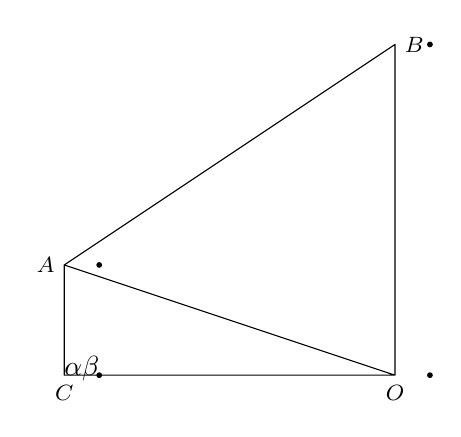
\begin{tikzpicture}[scale=0.7, line join=round, line cap=round,font=\footnotesize,>=stealth]
			\path (0,0)coordinate[label=below:$C$](C) (0,2)coordinate[label=left:$A$](A) (6,0)coordinate[label=below:$O$](O) (6,6)coordinate[label=right:$B$](B) ;
			\draw[line width=0.4pt,black] (A)--(C)--(O)--(B)--(A)--(O);
			\tkzMarkAngle[size=0.8cm](O,A,B)
			\tkzLabelAngle[pos = 0.3](O,A,B){$\alpha$}
			\tkzMarkAngle[size=0.7cm, mark=||,mksize=2cm](B,O,A)
			\tkzLabelAngle[pos = 0.3](B,O,A){$\beta$}
			\fill[black] (A)circle(1.5pt); 
			\fill[black] (C)circle(1.5pt);
			\fill[black] (B)circle(1.5pt);
			\fill[black] (O)circle(1.5pt);
		\end{tikzpicture}
	}
}
\end{ex}
\begin{ex}
	\immini{Muốn đo chiều cao của tháp Chàm Por Klong Garai ở Ninh Thuận người ta lấy hai điểm $A$, $B$ trên mặt đất có khoảng cách $AB=12m$ cùng thảng hàng với chân $C$ của tháp để đặt hai giác kế. Chân của giác kế có chiều cao $h=1{,}3 m$. Gọi $ D$ là đỉnh tháp và hai điểm $A'$, $B'$ cùng thẳng hàng với điểm $C'$ thuộc chiều cao $CD$ của tháp. Người ta đo được góc $\widehat{DA'C'}=49^{\circ}$ và góc $\widehat{DB'C'}=35^{\circ}$. Hãy tính chiều cao $CD=C'D+C'C$ của tháp đó.}{
			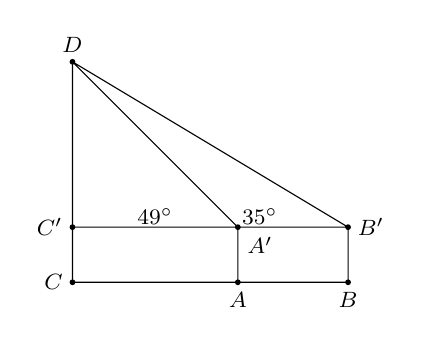
\begin{tikzpicture}[scale=0.7, line join=round, line cap=round,font=\footnotesize,>=stealth]
			\path (0,0)coordinate[label=left:$C$](C) (3,0)coordinate[label=below:$A$](A) (5,0)coordinate[label=below:$B$](B) (0,1)coordinate[label=left:$C'$](C') (3,1)coordinate[label=below right:$A'$](A') (5,1)coordinate[label=right:$B'$](B') (0,4)coordinate[label=above:$D$](D) ;
			\draw[line width=0.4pt,black] (C')--(C)--(A)--(B)--(B')--(A')--(C')--(D)--(A') (D)--(B') (A')--(A);
			\tkzMarkAngle[size=1.0cm](D,A',C');
			\node at (1.5,1.2) {$49^{\circ}$};
			\tkzMarkAngle[size=1.0cm,mark=||,mksize=2cm](D,B',C');
		   \node at (3.4,1.2) {$35^{\circ}$};
			\fill[black] (C')circle(1.5pt); 
			\fill[black] (D)circle(1.5pt);
			\fill[black] (A)circle(1.5pt); 
			\fill[black] (C)circle(1.5pt);
			\fill[black] (B)circle(1.5pt);
			\fill[black] (B')circle(1.5pt);
			\fill[black] (A')circle(1.5pt);			
		\end{tikzpicture}
		
	}	
	\choice
	{$30{,}7m$}
	{$25{,}7m$}
	{\True $32m$}
	{$31{,}7m$}

	\loigiai{	
		Ta có $CC'=1{,}3 m$.\\
		Khi đó, áp dụng định lý sin trong tam giác $A'B'D$ ta được\\ $\dfrac{B'D}{\sin(180^{\circ}-\widehat{DA'C'})}=\dfrac{A'B'}{\sin(180^{\circ}-\widehat{DA'C'}-35^{\circ})} \Leftrightarrow \dfrac{B'D}{\sin 131^{\circ}}=\dfrac{12}{\sin 14^{\circ}} \Leftrightarrow B'D=\dfrac{12\cdot \sin 131^{\circ}}{\sin 14^{\circ}}$ .\\
		Xét tam giác $ B'C'D$ có $C'D=B'D \cdot \cos 35^{\circ} \approx 30{,}7 m$.
	}
\end{ex}
\begin{ex}
Một cây cột điện cao $20 m$ được đóng trên một triền dốc thẳng nghiêng hợp với phương nằm ngang một góc $17^{\circ}$. Người ta nối một dây cáp từu đỉnh cột điện đến cuối dốc. Tìm chiều dài của dây cáp bết rằng đoạn đường từ đáy cọc đến cuối dốc bằng $72 m$.

	\choice
	{\True $83{,}4m$}
	{$34{,}7m$}
	{$75{,}3m$}
	{$71{,}7m$}
	\loigiai{		
		\immini{
		Ta có $\widehat{ACD}=180^{\circ} -(90^{\circ}-17^{\circ})=107 ^{\circ}$.\\
		Trong tam giác $ABC$ vuông tại $B$ có $AC=\dfrac{AB}{\cos 17^{\circ}} \approx 75{,}3 m$.\\
		ÁP dụng định lý Cosin trong tam giác $ACD$, ta có
\begin{align*}
			$AD^{2} &= AC^{2}+CD^{2}-2AC \cdot CD \cdot \cos \widehat{ACD}\\
		&= 75{,}3^{2}+20^{2}-2 \cdot 75{,}3 \cdot 20 \cdot \cos 107^{\circ} \approx 6950{,}7$.
	\end{align*}
		 $\Rightarrow AD\approx 83{,}4 m$.
	}{
	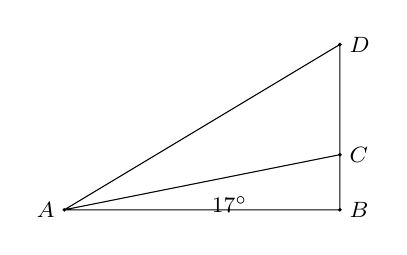
\begin{tikzpicture}[scale=0.7, line join=round, line cap=round,font=\footnotesize,>=stealth]
	\path (0,0)coordinate[label=left:$A$](A) (5,0)coordinate[label=right:$B$](B) (5,1)coordinate[label=right:$C$](C) (5,3)coordinate[label=right:$D$](D) ;
	\draw[line width=0.4pt,black] (C)--(A)--(B)--(C)--(D)--(A)--(C);
	\tkzMarkAngle[size=2.0cm](B,A,C);
	\node at (3,0.1) {$17^{\circ}$};

	\fill[black] (A)circle(1.0pt); 
		\fill[black] (B)circle(1.0pt);
	\fill[black] (C)circle(1.0pt);	\fill[black] (D)circle(1.0pt);

\end{tikzpicture}		
}	 
	}
\end{ex}
\begin{ex}
	\immini{Hai chiếc tàu thủy $P$ và $Q$ cách nhau $300m$. Từ $P$ và $Q$ thẳng hàng với chân $A$ của tháo hải đăng $AB$ ở trên bờ biển người ta nhìn chiều cao $AB$ của tháp dưới các góc $ \widehat{BPA}=35^{\circ}$, $\widehat{BQA}=48^{\circ}$. Tính chiều cao của tháp.}{
		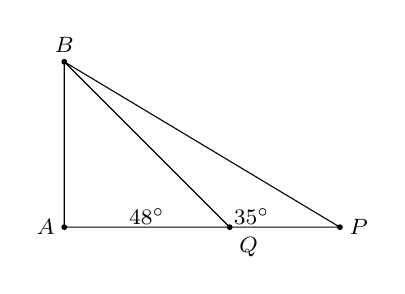
\begin{tikzpicture}[scale=0.7, line join=round, line cap=round,font=\footnotesize,>=stealth]
		\path  (0,1)coordinate[label=left:$A$](A) (3,1)coordinate[label=below right:$Q$](Q) (5,1)coordinate[label=right:$P$](P) (0,4)coordinate[label=above:$B$](B) ;
		\draw[line width=0.4pt,black] (B)--(A)--(Q)--(P)--(B)--(Q);
		\tkzMarkAngle[size=1.0cm](B,Q,A);
		\node at (1.5,1.2) {$48^{\circ}$};
		\tkzMarkAngle[size=1.0cm,mark=||,mksize=2cm](B,P,A);
		\node at (3.4,1.2) {$35^{\circ}$};
	
		\fill[black] (A)circle(1.5pt); 
			\fill[black] (B)circle(1.5pt);
		\fill[black] (P)circle(1.5pt);
		\fill[black] (Q)circle(1.5pt);			
	\end{tikzpicture}
	}
	
	\choice
	{\True $568{,}5m$}
	{$445{,}7m$}
	{$375{,}2m$}
	{$398{,}5m$}
	
	\loigiai{	
		Ta có $AQ=AB \cdot \cot 48^{\circ}$, $AP=AB \cdot \cot 35^{\circ}$.\\
		$PQ=AP-AQ=AB \cdot (\cot 35^{\circ}-\cot 48^{\circ})$.\\
	Suy ra $AB=\dfrac{PQ}{(\cot 35^{\circ}-\cot 48^{\circ})} \approx 568{,}5 m.$
		
	}
\end{ex}
\begin{ex}
Một hành khách ngồi trong một máy bay, bay ở độ cao 10 km nhìn xuống hai thị trấn dưới mặt đất. Góc hợp bởi phương ngang và hai thị trấn lần lượt là $28^{\circ}$ và $55^{\circ}$ (hình vẽ). Tính khoảng cách giữa hai thị trấn.
	\choice
	{\True $11{,}79km$}
	{$15{,}7km$}
	{$21{,}9km$}
	{$8{,}5km$}
	
	\loigiai{\immini{	
		Ta có $\widehat{CAD}=55^{\circ}-28^{\circ}=27^{\circ}$.\\
		Xét tam giác $ACO$ có $\widehat{OAC}=90^{\circ}-55^{\circ}=35^{\circ}$ và\\ $\cos \widehat{OAC}=\dfrac{AO}{AC} \Leftrightarrow AC=\dfrac{10}{\cos 35^{\circ}} \approx 12{,}2 km.$\\
		Áp dụng định lý sin trong tam giác $ACD$, ta có 
		\begin{center}
				$\dfrac{CD}{\sin 27^{\circ}}=\dfrac{AC}{\sin 28^{\circ}} \Leftrightarrow CD=\dfrac{12{,}2 \cdot \sin 27^{\circ}}{\sin 28^{\circ}} \approx 11{,}79 km$.
		\end{center}
Vậy khoảng cách hai thị trấn khoảng $11{,}79 km$.}{	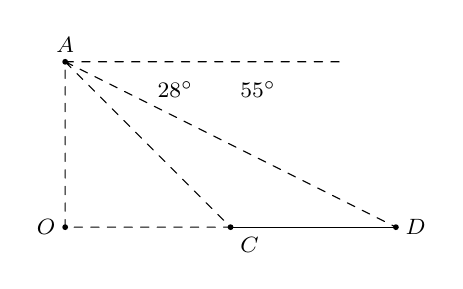
\begin{tikzpicture}[scale=0.7, line join=round, line cap=round,font=\footnotesize,>=stealth]
	\path  (0,1)coordinate[label=left:$O$](O) (3,1)coordinate[label=below right:$C$](C) (6,1)coordinate[label=right:$D$](D) (0,4)coordinate[label=above:$A$](A) ;
	\coordinate[label=right:$ $] (K)at(5,4);	
\draw[dashed,black] (A)--(C)--(O)--(A)--(D) (A)--(K);
\draw[line width=0.4pt,black] (C)--(D);
	\tkzMarkAngle[size=2.6cm](C,A,K);
	\node at (3.5,3.5) {$55^{\circ}$};
	\tkzMarkAngle[size=1.0cm,mark=||,mksize=2cm](D,A,K);
	\node at (2.0,3.5) {$28^{\circ}$};
	\fill[black] (A)circle(1.5pt); 
	\fill[black] (O)circle(1.5pt);
	\fill[black] (C)circle(1.5pt);
	\fill[black] (D)circle(1.5pt);			
\end{tikzpicture}}
		
	}
\end{ex}

\begin{ex}
	Ông Hùng dự định gửi vào ngân hàng một số tiền với lãi suất $6{,}5\%$ một năm. Biết rằng cứ sau mỗi năm số tiền lãi sẽ gộp vào vốn ban đầu. Số tiền $x$ (triệu đồng, $x\in\mathbb{N}$) nhỏ nhất mà ông Hùng cần gửi vào ngân hàng để sau ba năm (mới rút lãi) thì số tiền lãi có thể mua một chiếc xe máy trị giá $60$ triệu đồng là
	\choice
	{$280$}
	{\True $289$}
	{$300$}
	{$308$}
	\loigiai{
		Số tiền thu được sau ba năm (cả tiền lãi và tiền gốc) là $x(1+6{,}5\%)^3$.\\
		Ta có $x(1+6{,}5\%)^3-x=60\Rightarrow x\approx 289$ triệu đồng.}
\end{ex}

\begin{ex}
	Một bác nông dân vừa bán trâu được số tiền là $32\,000\,000$ đồng. Do chưa cần dùng đến số tiền nên bác nông dân mang toàn bộ số tiền đó đi gửi tiết kiệm loại kỳ hạn $6$ tháng vào ngân hàng với lãi suất $5{,}7\%$ một năm (lãi kép) thì sau $4$ năm $6$ tháng bác nông dân nhận được bao nhiêu tiền cả vốn lẫn lãi? (Biết rằng bác nông dân đó không rút cả vốn lẫn lãi tất cả các định kì trước).
	\choice
	{\True$41\,208\,674$ đồng}
	{$40\,208\,000$ đồng}
	{$48\,416\,000$ đồng}
	{$52\,701\,729$ đồng}
	\loigiai{ Lãi suất mỗi kỳ là $r=\dfrac{5{,}7}{2}\%=2{,}85\%$.\\
		$4$ năm $6$ tháng ứng với $n=9$ kỳ gửi. Tổng số tiền cả vốn và lãi thu được sau $9$ kỳ gửi là
		\[S=32\,000\,000(1+2{,}85\%)^9=41\,208\,674\,\,\text{đồng}.\]
	}
\end{ex}

\begin{ex}
	Kể từ ngày $1/1/2021$, cứ vào ngày mùng $1$ hàng tháng, ông $A$ ra gửi ngân hàng số tiền là $x$ (đồng) với lãi suất $0{,}5\%$/ tháng. Biết tiền lãi của tháng trước được cộng vào tiền gốc của tháng sau. Tìm giá trị nhỏ nhất của $x$ để đến ngày $1/1/2022$ khi ông $A$ rút cả gốc và lãi thì được số tiền lãi hơn $10$ triệu đồng? (Kết quả lấy làm tròn đến nghìn đồng).	
	\choice
	{$25173000$}
	{$21542000$}
	{$21541000$}
	{\True $25174000$}
	\loigiai{
		Số tiền mà ông $A$ nhận được gồm vốn và lãi sau $n$ tháng là
		$$\dfrac{x}{r}\left[(1+r)^{n+1}-1\right]-x$$ trong đó $r$ là lãi suất/tháng.\\	
		Theo đề bài ta có 
		\begin{eqnarray*}
			&&\dfrac{x}{0{,}5\%}\left[(1+0{,}5\%)^{12+1}-1\right]-x=12x+10000000\\
			&\Leftrightarrow& x=\dfrac{10000000}{200\cdot (1+0{,}5^{13})-200-13}\approx 25174000. 
		\end{eqnarray*}
	}
\end{ex}

\begin{ex}
Một người gửi tiền vào ngân hàng với lãi suất không thay đổi là $6\%$/ năm. Biết rằng nếu không rút tiền ra khỏi ngân hàng thì cứ sau mỗi năm, số tiền lãi sẽ được nhập vào vốn ban đầu (người ta gọi là lãi kép). Người đó định gửi tiền trong vòng $3$ năm, sau đó rút ra $500$ triệu đồng. Hỏi số tiền ít nhất người đó phải gửi trong ngân hàng (làm tròn đến hàng triệu) là bao nhiêu triệu đồng?
\choice
{\True $420$}
{$410$}
{$400$}
{$390$}
\loigiai{
Gọi $A$ là số tiền ban đầu cần gửi, $r=0{,}06$ là lãi suất hàng năm.\\
Sau $3$ năm, số tiền cả gốc lẫn lãi của người đó là 
$S=A(1+r)^3$.\\
Ta có $S\ge 500\Leftrightarrow A(1+r)^3\ge 500\Leftrightarrow A\ge \dfrac{500}{(1+r)^3}=\dfrac{500}{1{,06}^3}\approx 420$ triệu.
}
\end{ex}

\begin{ex}%[Khảo sát chất lượng lần 1, Trường THPT Triệu Sơn 3 - Thanh Hóa, 2021]%[Lê Hồng Phi, 12EX6]%[2D2B4-5]
Ông X gửi vào ngân hàng $60$ triệu đồng theo hình thức lãi kép. Lãi suất ngân hàng là  $8\%$ trên năm. Sau $5$ năm ông X tiếp tục gửi thêm $60$ triệu đồng nữa. Hỏi sau $10$ năm kể từ lần gửi đầu tiên ông X đến rút toàn bộ tiền gốc và tiền lãi được là bao nhiêu? (Biết lãi suất không thay đổi qua các năm ông X gửi tiền).
\choice
{\True $217{,}695$ (triệu đồng)}
{$231{,}815$ (triệu đồng)}
{$190{,}271$ (triệu đồng)}
{$197{,}201$ (triệu đồng)}
\loigiai
{Công thức tính tiền gốc lẫn lãi của hình thức gửi ngân hàng theo lãi kép là $T_n=A(1+r)^n$, trong đó $A$ là số tiền gửi ban đầu, $r$ là lãi suất hàng năm, $n$ là số năm gửi.\\
Vậy tổng số tiền ông X nhận được là $$60\cdot (1+0.08)^{10}+60\cdot (1+0.08)^5\approx 217{,}695\ (\text{triệu đồng}).$$
}
\end{ex}

\Closesolutionfile{ans}
\Closesolutionfile{ansbook}
% \indapan{10}{ans/ans-10-15}